\documentclass[a4paper,12pt,twoside]{report}
\usepackage[a4paper,width=150mm,top=25mm,bottom=25mm]{geometry}
\setlength{\headheight}{15pt}

\usepackage[utf8]{inputenc}
\usepackage{xspace}
\usepackage[portuguese]{babel}

% o comando say para referenciar texto
\usepackage{dirtytalk}

% melhor code blocks
\usepackage{listings}

% imagens floatuantes ao lado de texto
\usepackage{wrapfig}


% \usepackage{url}

% %% Define a new 'leo' style for the package that will use a smaller font.
% \makeatletter
% \def\url@leostyle{%
%   \@ifundefined{selectfont}{\def\UrlFont{\sf}}{\def\UrlFont{\small\ttfamily}}}
% \makeatother
% %% Now actually use the newly defined style.
% \urlstyle{leo}

%to ocupy all the space
% \newlength{\textundbildtextheight}
% \newcommand{\textundbild}[2]{\settototalheight\textundbildtextheight{\vbox{#1}}[#1]

%floats figures to stay in the place where they are declared(use H to use it exemple:
%\begin{figure}[H] 
%)
\usepackage{float}

%para tabelas ajustadas
\usepackage{tabularx}
\usepackage{booktabs}
\usepackage{array}
\newcolumntype{C}{>{\centering\arraybackslash}X}

%para que o primeiro paragrafo indente
\usepackage{indentfirst}

%para for loops
\usepackage{pgffor}

%para checar paginas em branco e virar
\usepackage[strict]{changepage}

%Fontes especias de matemática

\usepackage{amsfonts}

%hide hidelinks esconde os links There were undefined references \subsection{Arquitetura}de terem bordas feias
% backref para ter links entre refenrecias e toc
% hidelinks para nao aparecer a caixa azul
\usepackage[hidelinks]{hyperref}
% pacote para os headers e footers fixes
\usepackage{fancyhdr}

%para poder ter os compactitem lists
\usepackage{paralist}

%ter acesso a imagens
\usepackage{graphicx}
\usepackage{svg}
\graphicspath{{images/}{anexos/}}

\usepackage{nicematrix}

%printar pdfs
\usepackage{pdfpages}

%obter o nome de onde estao as referencias
\usepackage{nameref}

% package para tirar notas
\usepackage{easy-todo}

%cores lol
\usepackage{color, colortbl}

%para referenciar com o tipo
\usepackage[nameinlink]{cleveref}
\crefname{figure}{figura}{figuras}
\crefname{wrapfigure}{figura}{figuras}
\crefname{table}{tabela}{tabelas}
\crefname{chapter}{capítulo}{capítulos}
\crefname{subsection}{subsecção}{subsecções}



%using markdown
\usepackage[hashEnumerators,smartEllipses]{markdown}
%for instructions see https://pt.overleaf.com/learn/how-to/Writing_Markdown_in_LaTeX_Documents

\usepackage{csquotes}
\usepackage{setspace}
\usepackage{afterpage}
\usepackage{longtable}
% \usepackage{tightlist}
% CORES

%tratar das cores
\usepackage{xcolor}
\usepackage{pagecolor,lipsum}% http://ctan.org/pkg/{pagecolor,lipsum}
% \usepackage{memoir}
% definição de uma cor
% \definecolor{name}{model}{color-spec}
\definecolor{aquamarine}{rgb}{0, 181, 190}

% meter o fundo em pretos e os caracteres em branco
\pagecolor{black}
\color{white}
\newcommand{\linkcolor}{aquamarine}
%link color for white mode
% \newcommand{\linkcolor}{blue}

\usepackage{xcolor}

\usepackage{biblatex} %Imports biblatex package
\addbibresource{referencias.bib} %Import the bibliography file
% -------- Acrónimos ------------- %

%para os acrónimos
% usar \newacronym{⟨label⟩}{⟨abbrv⟩}{⟨full⟩} para fazer um
\usepackage[acronym,automake]{glossaries}
\makeglossaries
% \usepackage{glossary-longbooktabs}

%change the size of captions
\usepackage[font=small]{caption}
\captionsetup[wrapfigure]{font=scriptsize,justification=centering}

%\newglossary[slg]{glos}{Glossário}

% siglas
\newacronym{isec}{ISEC}{Instituto Superior de Engenharia de Coimbra}
\newacronym{ipc-education}{IPC (Educação)}{Instituto Politécnico de Coimbra}
\newacronym{ipc-compute}{IPC (Computação)}{\textit{Inter-Process Communication}}
\newacronym{ir}{IR}{\textit{Infrared}}
\newacronym{api}{API}{\textit{Application Programming Interface}}
\newacronym{ctesp}{CTeSP}{Curso Técnico Superior Profissional}
\newacronym{deis}{DEIS}{Departamento de Engenharia Informática e de Sistemas}
\newacronym{ide}{IDE}{\textit{Integrated Development Environment}}
\newacronym{bpm}{BPM}{\textit{Beats Per Minute}}
\newacronym{abi}{ABI}{\textit{Application Binary Interface}}
\newacronym{ms}{MS}{\textit{Microsoft}}
\newacronym{std}{std}{\textit{Standard Library}}
\newacronym{ipfs}{IPFS}{\textit{InterPlanetary File System}}
\newacronym{fs}{FS}{\textit{File System}}
\newacronym{pos}{PoS}{\textit{Proof of Stake}}
\newacronym{pow}{PoW}{\textit{Proof of Work}}
\newacronym{json}{JSON}{\textit{JavaScript Object Notation}}
\newacronym{raii}{RAII}{\textit{Resource Acquisition Is Initialization}}
\newacronym{nat}{NAT}{\textit{Network Address Translation}}
\newacronym{udp}{UDP}{\textit{User Datagram Protocol}}
\newacronym{voip}{VoIP}{\textit{Voice over Internet Protocol}}
\newacronym{p2p}{P2P}{\textit{Peer-to-peer}}
\newacronym{cpu}{CPU}{\textit{Central processing unit}}
\newacronym{nfc}{NFC}{\textit{Near-Field Communication}}
\newacronym{fps}{FPS}{\textit{Frames Per Second}}
\newacronym{soa}{SOA}{Service-oriented architecture}

%glossario
\newglossaryentry{bitcoin}{
	name=Bitcoin,
	description = {Uma criptomoeda descentralizada, sendo um dinheiro eletrônico para transações ponto a ponto\cite{bitcoin_wiki}}
}

\newglossaryentry{blockchain}{
	name={blockchain},
	description={Uma tecnologia de registro distribuído que visa a descentralização como medida de segurança\cite{blockchain_wiki}}
}

\newglossaryentry{twitter}{
	name = Twitter,
	description = {Rede social para \textit{microblogging}\cite{twitter_wiki}}
}

\newglossaryentry{switch}{
	name={Nintendo Switch},
	description={consola de jogos de vídeo híbrida produzida pela empresa Nintendo\cite{switch_wiki}}
}

\newglossaryentry{gc}{
	name={garbage collector},
	description={processo usado para a automatização do gestor de memória\cite{gc_wiki}}
}

\newglossaryentry{data-race}{
	name={\textit{data race}},
	description={ocorrência de múltiplas linhas de execução acederem ao mesmo espaço de memoria sem a apropriada sincronização e pelo menos uma escrita nesse espaço}
}

\newglossaryentry{gateway}{
	name={gateway},
	description={peça de \textit{networking hardware} ou \textit{software} usado em telecomunicações\cite{gateway_wiki}}
}

\newglossaryentry{anticheat}{name={Anti-cheat},description={software que tenta prevenir fraudes em  jogos de vídeo}}

\newglossaryentry{pay2win}{name={pay-to-win},description={jogos que deixam o jogador usar dinheiro usado no mundo real para ter vantagem dentro do mundo do jogo \cite{pay2win}}}

% ----------- MACROS --------------- %

\newcommand{\myemptypage}{
    \newpage
    \null
    \thispagestyle{empty}
    %\addtocounter{page}{-1}
    \newpage
}

\newcommand{\nextpage}{
\clearpage
\newpage
\mbox{~}
\clearpage
\newpage
}

\newcommand{\clearforchapter}{\clearpage~\thispagestyle{cleared}\cleartorecto}

\newcommand{\checkandnewpageifeven}{
    \newpage
    \checkoddpage{}
    \ifoddpage{} \else \nextpage{} \fi
}

\newcommand{\lk}[2]{\href{#1}{\textcolor{\linkcolor}{#2}}}

\newcommand{\chapterf}[1]{
    \checkandnewpageifeven{}
    \chapter{#1}
    \thispagestyle{fancy}
}

\newcommand{\mytitle}{Game Chaining}
\newcommand{\gamechaining}{\textit{\mytitle{}}}

% set dos headers e footers
\pagestyle{fancy}
\fancyhf{}
\lhead{\mytitle{}}
\rhead {\thechapter}
\fancyfoot[LE,RO]{\thepage}
% \rfoot{\thepage}

%set do espaçamento entre linhas
\setstretch{1.25}
%set indentação
\setlength\parindent{0.75cm}

%set font family to arial
\usepackage{helvet}
\renewcommand{\familydefault}{\sfdefault}
% \newcommand\todo[1]{\textbf{\textcolor{red}{#1}}}
% comment this to hide todos
% \renewcommand\todo[1]{}

% troca os cites por subercites
% \renewcommand{\cite}[1]{\supercite{#1}}
% mete os parentices retos nos supercites
% \DeclareCiteCommand{\supercite}[\mkbibsuperscript]
%   {\iffieldundef{prenote}
%      {}
%      {\BibliographyWarning{Ignoring prenote argument}}%
%    \iffieldundef{postnote}
%      {}
%      {\BibliographyWarning{Ignoring postnote argument}}}
%   {\usebibmacro{citeindex}%
%    \bibopenbracket\usebibmacro{cite}\bibclosebracket}
%   {\supercitedelim}
%   {}


\addto\captionsportuguese{% Replace "english" with the language you use
  \renewcommand{\contentsname}%
    {Índice}%
}



% transforma todos os gls para itálico
\renewcommand{\glstextformat}[1]{\textit{#1}}

% ======== APAGAR OS TODOS =============
% \renewcommand\todo[1][]{}
% \renewcommand\listoftodos{}

% --------  DOCUMENTO

\begin{document}
\pagenumbering{roman}

\begin{titlepage}
    
    \noindent
        \includegraphics[height=2cm]{images/NMlogo_colour.png} 
        \hfill{}
        \includegraphics[height=2cm]{images/logo-isec-transparente.png}
        
        \begin{center}
        \begin{large}
            \vfill{}
            \textbf{\huge{\mytitle{}}}\\
            \vspace{10px}
            
            \begin{Large}
                
                Relatório de Estágio
                \vfill
                João Pedro Neves Gonçalves\\
                2018014306
                
            \end{Large}
            \vfill
            Orientadores:

            Prof. Anabela Jesus Gomes  \(|\) ISEC\\
            Diogo Vasconcelos \(|\) Nerd Monkeys\\
            Alexandre Barbosa \(|\) Nerd Monkeys

            \vfill
            Licenciatura em Engenharia Informática\\
            Ramo de Desenvolvimento de Aplicações\\
            Instituto Superior de Engenharia de Coimbra\\
            Instituto Politécnico de Coimbra
            
           \vfill{}
            Setembro de 2021
        \end{large}
    \end{center}
\end{titlepage}
\myemptypage
\setcounter{page}{1}
% \checkandnewpageifeven
\section*{Agradecimentos}
% \addcontentsline{toc}{section}{\protect\numberline{}Agradecimentos}

Começo já a agradecer ao \acrfull{isec} pelo ensino, aprendi muito nestes 3 anos
tudo graças, não só aos professores, muitos dos quais estavam sempre
disponíveis a ensinar, como também aos colegas que encontrei, que me
ajudaram e apoiaram.
Agradeço especialmente à minha orientadora Anabela Jesus Gomes que estava sempre disponível para ajudar.

Agradeço a todas as equipas na Nerd Monkeys, especialmente a minha Team
7, Team Patas e à Team Golden Snub.

Quero agradecer em especial ao Alexandre Barbosa por me ter integrado na
empresa e ajudar em tudo o que era preciso, ao Diogo Vasconcelos que
me orientou e apoiou em todo o meu percurso, ao Iuri Martinho por
insistir comigo e ajudar-me no que era preciso e à Mafalda Duarte.

Agradeço aos meus colegas de curso Ana Filipa Alves, Marco Domingues,
Eduardo Pina e Rafaela Santos pela ajuda e apoio ao longo desta jornada.

Por último, gostaria de agradecer à minha família por ter-me dado o apoio necessário.



% \newpage
\checkandnewpageifeven
\section*{Resumo}
% \addcontentsline{toc}{section}{\protect\numberline{}Resumo}

No mundo dos jogos de vídeo, têm vindo a ser experimentadas variadas tecnologias, sendo as mesmas posteriormente evoluídas de forma a melhor satisfazerem o objetivo da sua utilização.

A \textit{Nerd Monkeys}, uma empresa desenvolvedora de jogos de vídeo com interesse em explorar novas tecnologias, foi a empresa onde o estágio apresentado neste trabalho se desenvolveu.

A primeira tecnologia usada no estágio foi a \textit{blockchain}, tal como estava planeado na proposta de estagio. 
Relativamente ao \textit{blockchain} foi maioritariamente estudada a tecnologia subjacente, o seu modo de funcionamento, os seus protocolos e as suas aplicações genéricas e concretamente nos jogos de vídeo.

Para experimentar alguns dos conceitos acumulados na pesquisa sobre \textit{blockchain} foi realizado um projeto designado de \textit{AC7ION} do tipo servidor-cliente. Ambos foram desenvolvidos em \textit{Rust}. O servidor faz a troca de informações com a \acrfull{api} do \textit{Twitter}. Este servidor envia os \textit{tweets} obtidos da \acrshort{api} para uma biblioteca partilhada quando requisitados. A biblioteca pode ser usada por qualquer \textit{game engine} que suporte uma \acrfull{abi} para a linguagem \textit{C}.

O último projeto efetuado foi um detetor de batimentos cardíacos com o sensor de \acrfull{ir} da \gls{switch} desenvolvido em \textit{C++}. Este teve como objetivo dar a conhecer o \textit{hardware} e \textit{software} desta consola de jogos de vídeo, permitindo conhecer o espaço de desenvolvimento de uma consola e o que pode ser nela usado e desenvolvido.

\textit{\textbf{Palavras-chave:} Blockchain, Rust, \acrshort{ir} Sensor, Jogos de vídeo}

% \newpage
\checkandnewpageifeven
\section*{Abstract}

Various technologies are tried out in the world of video games,
being later evolved in ways to better satisfy
the purpose of its use.

Nerd Monkeys, the company where the internship took place, is a video game developer company that has
the interest in exploring new technologies.

The first technology used in the internship was blockchain, as it was
planned in the internship proposal. For the blockchain it was essentially explored its underlying technology, its working mode, its protocols and its general and specific applications in video games.

To try out some of the concepts accumulated in the blockchain research
a server-client type program was performed. Both developed in Rust for exchanging information with the Twitter API. This program sends the information obtained from the API to a shared library. The shared library, also performed at this stage can be used by any game engine that supports an ABI for the C language.


The last project carried out was a heart beats detector for Nintendo Switch IR sensor developed in C++. This was developed to make known the hardware and software of this video games console allowing to know its development space and what can be used on it.

\textit{\textbf{Keywords:} Blockchain, Rust, \acrshort{ir} Sensor, Video Games}

% \newpage

    \checkandnewpageifeven
\tableofcontents{}

\checkandnewpageifeven
\listoffigures{}

\checkandnewpageifeven
\checkandnewpageifeven
\listoftables{}

\checkandnewpageifeven
\printacronyms[title=Abreviaturas]
\printglossary



% CONTEUDOS PRINCIPAIS
\newpage
\checkoddpage{}
\pagenumbering{arabic}
\ifoddpage
    \setcounter{page}{1}
\else
    \setcounter{page}{0}
    \myemptypage
\fi

\chapterf{Introdução}


\label{chap:introducao}

Na área dos jogos de vídeo várias são as tecnologias exploradas de forma a melhorar as experiências dos utilizadores ao jogar.

O trabalho apresentado no presente relatório representa também uma contribuição nesta temática. Consiste numa sumarização do
trabalho desenvolvido, tanto a nível teórico como prático, no estágio curricular no âmbito da unidade curricular de Projeto ou Estágio na empresa
Nerd Monkeys, de 1 de março de 2021 a 18 de julho de 2021, para efeitos de conclusão da
Licenciatura de Engenharia Informática, do \acrfull{isec}.

Neste capítulo, é apresentado o contexto do estágio, os seus objetivos,
entidades envolvidas na realização do mesmo, bem como a estrutura do relatório.

\section{Instituto Superior de Engenharia de Coimbra}

O \acrshort{isec} é uma das
unidades constituintes do \gls{ipc-education}. A
missão do \gls{ipc-education} corresponde à criação, transmissão e difusão de cultura, ciência e tecnologia. Para isso, é ministrada formação de nível superior para o exercício de atividades profissionais no domínio da Engenharia,
promovendo o desenvolvimento da região em que se insere. Foi fundado em
1974, tendo sido adicionado ao \acrshort{ipc-education} em 1988.

O \acrshort{ipc-education} tem uma variada oferta formativa disponível ao nível de mestrados, licenciaturas e \acrfull{ctesp}. O \acrfull{deis} dedica-se, desde 1989, à formação, investigação, desenvolvimento e prestação de serviços na área da Engenharia Informática. O \acrshort{isec} prima pelo caráter prático dos cursos que ministra, traduzido pelo elevado número de aulas laboratoriais, projetos e estágios o que, aliado à qualidade científica e pedagógica, resulta num elevado índice de empregabilidade.
\cite{isec_wiki}

\section{Nerd Monkeys}

A Nerd Monkeys foi fundada em 2013 por Diogo Vasconcelos e Filipe Duarte Pina \cite{nerdmonkeys_interview_eurogamerpt}. A empresa desenvolve e publica jogos, pelo que está sempre a investir em novas ideias para um jogo, tanto em histórias como tecnologias e paradigmas.

Como exemplo de jogos desenvolvidos na \textit{Nerd Monkeys} podem ser citados os jogos  ``\textit{Inspector Zé e Robot Palhaço em: Crime no Hotel Lisboa}'' (2014), ``\textit{Inspector Zé e Robot Palhaço em: O Assassino do Intercidades}'' (2018), ``\textit{Out of Line}'' (2021) e o ``\textit{Monkey Split}'' (2021) \cite{nerd_games_steam} publicados na Steam, uma plataforma de distribuição e venda de jogos.

A empresa também tem um histórico de adaptar jogos para a \gls{switch}, dos quais são exemplos os jogos ``\textit{Inspector Zé e Robot Palhaço em: Crime no Hotel Lisboa}''\cite{ze_eshop}, 
e um jogo de outro programador publicado pela \textit{Nerd Monkeys} cujo o nome do jogo é ``\textit{Traffix}'' \cite{traffix_eshop}. Porém, uma das áreas que a empresa quer explorar é a aplicação de \textit{blockchain} em jogos \textit{online}. Neste sentido, o estágio decorre no contexto da pesquisa de novas tecnologias para usar em novos jogos, neste caso especifico utilizando \textit{blockchain}.

\section{Proposta de Estágio}

A proposta de estágio (\hyperref[anexo:A]{anexo A}) elaborada pela \textit{Nerd Monkeys} visou a investigação da aplicação de \textit{blockchain} em jogos de vídeo, com a adição da utilização do motor de jogo \textit{Unreal Engine} com \textit{C++}.

O planeamento do desenvolvimento ficou divido nas seguintes tarefas:

\begin{itemize}
    \item T1 - Pesquisa e experiência prática – Durante este período o estagiário deverá realizar
    uma pesquisa extensiva sobre todas as componentes envolvidas no projeto e
    experimentação prática para validar os resultados da pesquisa. (5 semanas)

    \item T2 - Criação de ferramentas - tendo em vista as etapas T3 e T4. (4 semanas)

    \item T3 - Criação de protótipo – Criar um protótipo com base na pesquisa desenvolvida com um objetivo definido pelo orientador.(3 semanas)

     \item T4 - Desenvolvimento do videojogo – Com base no protótipo e ferramentas criadas deverá ser desenvolvido um videojogo em, pelo menos, formato de vertical \textit{slice} (demonstração jogável de todas as mecânicas). (10 semanas)

    \item T5 - Elaboração de relatório de estágio. (2 semanas)
\end{itemize}

O planeamento temporal das várias fases é apresentado na \cref{tab:diagrama-temporal}.

\begin{table}[H]
  \centering
  \footnotesize
  \def\arraystretch{2}
  \setlength\tabcolsep{3pt}
  \begin{tabularx}{\textwidth}
  {l*{24}{c}}
  \multicolumn{25}{c}{\textbf{Semanas}}\\
    &
    \multicolumn{1}{c}{01}&
    \multicolumn{1}{c}{02}&
    \multicolumn{1}{c}{03}&
    \multicolumn{1}{c}{04}&
    \multicolumn{1}{c}{05}&
    \multicolumn{1}{c}{06}&
    \multicolumn{1}{c}{07}&
    \multicolumn{1}{c}{08}&
    \multicolumn{1}{c}{09}&
    \multicolumn{1}{c}{10}&
    \multicolumn{1}{c}{11}&
    \multicolumn{1}{c}{12}&
    \multicolumn{1}{c}{13}&
    \multicolumn{1}{c}{14}&
    \multicolumn{1}{c}{15}&
    \multicolumn{1}{c}{16}&
    \multicolumn{1}{c}{17}&
    \multicolumn{1}{c}{18}&
    \multicolumn{1}{c}{19}&
    \multicolumn{1}{c}{20}&
    \multicolumn{1}{c}{21}&
    \multicolumn{1}{c}{22}&
    \multicolumn{1}{c}{23}&
    \multicolumn{1}{c}{24}
    \tabularnewline 
    T1 &
    \cellcolor{blue}{}&\cellcolor{blue}{}&
    \cellcolor{blue}{}&\cellcolor{blue}{}&
    \cellcolor{blue}{}&\\
    T2 &
    &&&&&
    \cellcolor{blue}{}&\cellcolor{blue}{}&
    \cellcolor{blue}{}&\cellcolor{blue}{}&\\
    T3 &
    &&&&&&&&&
    \cellcolor{blue}{}&\cellcolor{blue}{}&
    \cellcolor{blue}{}&\\
    T4 &
    &&&&&&&&&&&&
    \cellcolor{blue}{}&\cellcolor{blue}{}&
    \cellcolor{blue}{}&\cellcolor{blue}{}&
    \cellcolor{blue}{}&\cellcolor{blue}{}&
    \cellcolor{blue}{}&\cellcolor{blue}{}&
    \cellcolor{blue}{}&\cellcolor{blue}{}&\\
    T5 &
    &&&&&&&&&&&&&&&&&&&&&&
    \cellcolor{blue}{}&\cellcolor{blue}{}
  \end{tabularx}
  \caption{Diagrama de Gantt representativo do planeamento temporal}
  \label{tab:diagrama-temporal}
\end{table}

\section{Objetivos e Plano de Trabalhos}

Os objetivos iniciais deste trabalho, consistiam em aferir as capacidades da tecnologia \textit{blockchain} para além da sua utilização comum atual e aplicação concreta em jogos de vídeo com a subsequente criação de um prototipo funcional. Porém, foi considerado de interesse que o trabalho fosse principalmente de pesquisa, dadas as enormes capacidades e potencialidades desta tecnologia e assim aferir quais as melhores opções para a aplicar no contexto da empresa.

\section{Estrutura do relatório}

Este documento, para além da introdução, é composto pelos seguintes capítulos:

\begin{itemize}
    \item \Cref{chap:introducao} - Este é o primeiro capítulo, começa com a descrição da entidade de acolhimento e da instituição de ensino, seguindo-se a apresentação da proposta de estágio, os objetivos definidos e plano de trabalhos. Termina com esta secção que descreve a estrutura do relatório, bem como, a metodologia e notas extras.
    
    \item \Cref{chap:blockchain} - Neste capítulo é realizada a apresentação da primeira parte do estágio, onde foi realizada pesquisa sobre o tema de \textit{blockchain}. É realizada a descrição das várias tecnologias relacionadas com \textit{blockchain}, bem como análises e conclusões de como estas podem ser aplicadas num jogo.

    \item \Cref{chap:ac7ion} - Este capítulo apresenta a segunda parte do estágio, onde é relatado o desenvolvimento de um programa denominado \textit{AC7ION}. A função deste programa é a de receber \textit{tweets} para serem enviados a um cliente que faz comunicação com jogos.

    \item \Cref{chap:bpm} - Este capítulo apresenta a terceira parte do estágio, onde foi desenvolvido um detector de batimentos cardíacos, para a \textit{Nintendo Switch}, que usa o \acrfull{ir} Sensor desta para os detetar.

    \item \Cref{chap:conclusao} - Este capítulo trata da conclusão. No mesmo são tecidas algumas ideias finais sobre o trabalho desenvolvido e é analisado o sucesso do trabalho realizado.
\end{itemize}

Em complemento e como suporte de informação a estes capítulos, são também apresentadas \hyperref[bibliografia]{as referências bibliográficas} e um
 \hyperref[chap:anexos]{anexo}, estes podem ser vistos no final do documento.

\section{Metodologia e Notas Extras}

Os projetos aqui apresentados foram todos desenvolvidos como projetos internos da \textit{Nerd Monkeys}. Em projetos internos da empresa os membros das equipas têm grande liberdade criativa, o que significa que todos têm a liberdade de discutir e mudar o rumo do que está a ser desenvolvido se assim o líder do projeto concordar e for bem justificado.

Sendo que a metodologia de desenvolvimento era ágil e comparável com a \textit{Extreme Programming}, em que existe constante \textit{feedback}, reuniões todos os dias, em que a equipa está em constante contacto.

Os requisitos descritos nos vários capítulos foram inseridos com o propósito de definir os objetivos do trabalho a realizar. Tendo isso em conta, esses requisitos servem apenas como guias/
ideias base, pelo que podem não ser seguidos à risca durante o processo de desenvolvimento.



% !TeX root = ../relatorio-estagio.tex
\chapterf{Blockchain}
\label{chap:blockchain}

\section{Introdução}

Como requerido na \hyperref[anexo:A]{proposta de estágio} este trabalho centrou-se na pesquisa de \textit{blockchain}. O objetivo desta pesquisa foi de averiguar a pertinência e possibilidades da área de \textit{blockchain} e do mundo de tecnologias descentralizadas para a área dos jogos de vídeo. Esta pesquisa permitiria concluir se é possível ou não desenvolver jogos descentralizados baseados em \textit{blockchain} em que estes só precisam do poder computacional dos dispositivos dos jogadores para fazer verificação de dados e transições num jogo \textit{online}.

Os jogos feitos com o projeto \gamechaining{} devem ser o menos centralizados possível, reduzindo a utilização de servidores da empresa, permitindo que seja a comunidade do jogo a gerir os servidores do mesmo. Este tipo de independência não permite a utilização de mecanismos de \gls{pay2win}, sendo que a empresa só lucrará com a compra dos conteúdos dos jogos como música, modelos, texturas e outros.

O capítulo divide-se em várias partes, sendo estas:

\begin{itemize}
  \item \underline{\nameref{sec:blockchain_what}} - Nesta secção é explicado o conceito de \textit{blockchain} e termos relacionados.
  
  \item \underline{\nameref{sec:blockchain_where}} - Nesta secção é listada a maneira como esta tecnologia é usada no mercado.
  \item \underline{\nameref{sec:blockchain_how}} - Nesta secção é indicada a forma como a tecnologia \textit{blockchain} pode ser aplicada em jogos de vídeo.
  \item \underline{\nameref{sec:blockchain_conclusao}} - Nesta secção podem ser vistas conclusões sobre os assuntos expostos neste capítulo.
\end{itemize}
\newpage
\section{O que é \textit{blockchain}?}
\label{sec:blockchain_what}

Na sua aplicação mais básica é um conceito bastante simples de explicar:

``\textit{Blockchain é um tipo de Base de Dados Distribuída que guarda um registo de transações permanente e à prova de violação. Uma base de dados em blockchain consiste em dois tipos de registos: transações individuais e blocos.}

\textit{Um bloco é a parte concreta da blockchain onde são registadas algumas ou todas as transações mais recentes e uma vez concluídas são guardadas na blockchain como base de dados permanente. Sempre que um bloco é concluído um novo é gerado. Existe um número incontável de blocos na blockchain que são ligados uns aos outros - como uma cadeia - onde cada bloco contém uma referência para o bloco anterior.}'' \cite{blockchain_wiki}

Duma forma mais visual pode se usar o esquema referido na \cref{fig:blockchain-bitcoin-overview}, em que cada bloco contem o \textit{hash} do bloco anterior e a raiz da \textit{Merkle Tree}, que é uma árvore de \textit{hashs} para indexar o conteúdo.

\begin{figure}[!h]
  \centering
    \includegraphics[width=0.9\textwidth]{bitcoin-blockchain-simplefied.png}
  \caption{Visão geral do \textit{blockchain} no \textit{Bitcoin} \cite{bitcoin_devguide_blockchain}}
 \label{fig:blockchain-bitcoin-overview}
\end{figure}

O conceito de \textit{blockchain} foi introduzido por David Chaum em 1982 \cite{blockchain_origem} e foi conceptualizado por uma pessoa ou grupo conhecido como "Satoshi Nakamoto" em 2008 que publicou o design e implementação do que hoje é conhecido como \textit{Bitcoin}. \cite{blockchain_nakamoto}
% !TeX root = ../relatorio-estagio.tex

\newpage
\section{Como \textit{Blockchain} é aplicado no mercado?}
\label{sec:blockchain_where}

No mercado existe uma grande variedade de implementações de \textit{blockchain}. Algumas implementações são aplicadas como bases de dados, sendo que outras são aplicadas como criptomoedas.

\subsection{Criptomoedas}

Criptomoedas são a forma mais popular de usar \textit{blockchain}. Existe um grande número de criptomoedas, porém baseiam-se num conceito base que foi evoluindo. Devido à evolução da ideia, criptomoedas podem-se separar em 3 gerações: ouro digital, contratos inteligentes e escalabilidade.

\subsubsection{\textit{Bitcoin}: Ouro Digital}

\begin{wrapfigure}{r}{2cm}
    \includegraphics[width=2cm]{images/bitcoin.png}
    \caption{Logótipo do Bitcoin}
    \label{fig:bitcoin-logo}
\end{wrapfigure}

A primeira geração de criptomoedas é a aplicação de \textit{blockchain} para fins monetários, sendo o maior exemplo desta aplicação a criptomoeda \textit{Bitcoin} (\cref{fig:bitcoin-logo}).

``\textit{Bitcoin é uma criptomoeda descentralizada, sendo um dinheiro eletrónico para transações ponto-a-ponto. O primeiro artigo descrevendo uma implementação do Bitcoin foi criado em 2008 sendo apresentado no começo de 2009 a lista de discussão \textit{The Cryptography Mailing} por um programador ou grupo de programadores sob o pseudónimo Satoshi Nakamoto. Bitcoin é considerada a primeira moeda digital mundial descentralizada, constituindo um sistema económico alternativo, e responsável pelo ressurgimento do sistema bancário livre.}'' \cite{bitcoin_wiki}

\subsubsection{\textit{Ethereum}: Contratos Inteligentes}
\begin{wrapfigure}{r}{2cm}
    \includegraphics[width=2cm]{images/ethereum.png}
    \caption{Logótipo do Ethereum}
    \label{fig:ethereum-logo}
\end{wrapfigure}

\textit{Ethereum} (\cref{fig:ethereum-logo}) é uma criptomoeda conceptualizada em 2013, inicializada em 2015 por Vitalik Buterin. Esta tem a especificidade de ter capacidade de executar contratos inteligentes e é a segunda cropitomoeda mais valorizada, estando atrás de \textit{Bitcoin}, no que toca a valor de mercado. \cite{ethereum_wiki}

Um contrato inteligente é um protocolo de computador auto executável criado com a popularização das criptomoedas. Contratos inteligentes são feitos para facilitar e reforçar a negociação ou desempenho de um contrato, proporcionando confiança em transações \textit{online}. Contratos inteligentes permitem que pessoas desconhecidas façam negócios de confiança entre si, pela Internet, sem a necessidade de intermédio de uma autoridade central.

\textit{Ethereum} também começou a implementação do seu \textit{upgrade}, chamado de \textit{Ethereum 2.0}, que inclui  técnologias como \acrfull{pos} e \textit{sharding}, que serão analisada em mais detalhe nas subsecções \ref{concenso} e \ref{sharding} respectivamente. 

\subsubsection{\textit{IOTA}: Escalabilidade}

\begin{wrapfigure}{r}{2cm}
    \includegraphics[width=2cm]{images/iota.png}
    \caption{Logótipo do IOTA}
    \label{fig:iota-logo}
\end{wrapfigure}

Publicada em 2016 por Serguei Popov e com o propósito de resolver o problema de baixo número de transações por segundo, \cite{iota_wiki} , \textit{IOTA}  (\cref{fig:iota-logo}) baseia se na ideia de \textit{Tangle}, isto é, em vez de usar uma \textit{blockchain} com uma única linha de blocos usa grafos acíclicos dirigidos.

Nesta rede não existem mineiros, a verificação de cada transição é feita
pelos dois nós anteriores. \cite{directed_acyclic_graph} Explicando de uma forma mais visual, pode se verificar na \cref{fig:linevsdag} que numa \textit{blockchain} normal, são adicionados blocos um a um sendo que 51\% da rede tem de estar em concordância resultando numa velocidade constante. No caso da \textit{IOTA} a velocidade estala com o número de blocos na rede já que blocos podem ser verificados em paralelo.


Para se alcançar consenso existe uma entidade central da fundação \textit{IOTA} que faz transições sem valor para verificar se os nós são legítimos.

\textit{IOTA} tem a desvantagem de ser centralizada pelo facto de ter
coordenadores que são entidades confiadas e centralizadas.

\begin{figure}[!ht]
    \centering
    \includegraphics[width=\textwidth]{images/linevsdag.png}
    \caption{Uma \textit{Blockchain} comum comparada com o \textit{Tangle} do \textit{IOTA} (editada) \cite{iota_wiki}}
    \label{fig:linevsdag}
\end{figure}

\newpage
\subsection{Consensos}
\label{concenso}

\say{\textit{Um problema fundamental em sistemas de processamento distribuído é alcançar a confiança geral do sistema com a existência de processos defeituosos. Ademais, isso, normalmente, requer que processos concordem que algum dado ou valor seja necessário durante uma computação. Exemplos de aplicações de consenso distribuído incluem confirmar ou não uma transação para uma base de dados indefinida e concordar em relação à identidade de um líder.}}
 \cite{consensus_wiki}

Noutras palavras \textit{concensus} ou consenso na área da computação é o processo de confirmar que existe uma percentagem mínima de aplicações na rede que concordam com uma certa informação.

Existem vários algoritmos que podem fazer esse trabalho sendo que os de seguida apresentados parecem ser os mais utilizados:

\begin{itemize}
  \item
  \gls{pow} - é um sistema que cria um problema computacional
  cuja resolução tem um elevado custo de processamento mas é fácil de verificar. Como exemplo de implementação desta teoria refira-se a heurística de \textit{Fiat-Shamir} \cite{fiat-shamir_heuristic_wiki} 
  e o \textit{hashcash} que é o algoritmo usado pelo \textit{Bitcoin}. \cite{hashcash_wiki} É se chamado aqueles que fazem as verificações de mineiros. \cite{miners}

\item
  \gls{pos} - é um sistema que, em vez de criar um problema
  computacional para se verificar uma transição, coloca em causa o
  dinheiro daqueles que querem verificar. Se alguém quiser manipular de
  forma maliciosa uma transação terá, não só de ter 51\% do dinheiro que
  existe numa \textit{blockchain}, como também deve estar pronto a arriscar perder
  o dinheiro e fazer o seu valor descer, desencorajando assim ataques por causa do alto risco.
  Outra vantagem reside no facto de não ser preciso dispositivos de alto poder computacional para efetuar verificações. \cite{proof-of-stake}
  
\end{itemize}

\subsection{\textit{Sharding}}
\label{sharding}
\textit{Sharding} é o conceito de subdividir uma base de dados para que se melhore a sua escalabilidade. Isto é, quanto maior for o número de utilizadores na rede, melhor deve ser a divisão de trabalho. No contexto de \textit{blockchain}, quanto maior o número de utilizadores, maior o número de transições por segundo. \cite{sharding_geeks}

A implementação de \textit{sharding} é mais comum em bases de dados e criptomoedas com entidades confiadas pela rede como \textit{IOTA}, sendo a presença de \textit{sharding}  em criptomoedas públicas e descentralizadas sem elementos confiados ou favorecidos muito menos comum.

\subsection{Framework e Protocolos}

Também foram encontradas várias aplicações e \textit{frameworks} que podiam ser utilizadas ou poderiam servir como inspiração para aplicar no projeto. Uma lista dessa aplicações/ \textit{frameworks} poderá ser vista na tabela \ref{table:frameworks}.

\begin{table}[h!]
  \centering
  \begin{tabularx}{\linewidth}{>{\hsize=.3\hsize}lX}
    \multicolumn{1}{c}{\textbf{Nome}} & 
    \multicolumn{1}{c}{\textbf{Descrição}}
    \tabularnewline \tabularnewline 
    \textit{Hyperledger}&
    Uma \textit{pool} de projetos, apoiada pela \textit{Linux foundation}, relacionados com \textit{blockchain}. \cite{hyperledger}
    \tabularnewline \midrule
    \textit{BigchainDB}&
    Base de dados em \textit{blockchain}. Construída com base em \textit{consensus} de um líder. \cite{bigchaindb}
    \tabularnewline \midrule
    \acrfull{ipfs}&
    ``\textit{Sistema de Ficheiros Interplanetário é um protocolo e uma rede projetada para criar um armazenamento associativo ponto-a-ponto endereçável ao conteúdo de armazenamento e compartimentação, de hipermédia, num sistema de ficheiros distribuído.}'' \cite{ipfs_wiki}
    \tabularnewline \midrule
    \textit{Ethereum Casper}&
    \textit{Casper} é o protocolo que os pesquisadores de \textit{Ethereum} estão a estudar e a desenvolver para implementar \acrshort{pos} e \textit{sharding} em \textit{Ethereum}. \cite{ethereum_casper}
    \tabularnewline \midrule
    \end{tabularx}
  \caption{\textit{Frameworks} e Protocolos}
  \label{table:frameworks}
\end{table}

\newpage
\section{Como aplicar Blockchain no contexto de um jogo de vídeo?}
\label{sec:blockchain_how}

Nesta secção é indicada a forma como a tecnologia \textit{blockchain} pode ser aplicada em jogos de vídeo.

\subsection{Mercado Existente}

No mercado de jogos de vídeo, a aplicação de \textit{blockchain}
encontrava-se maioritariamente em jogos que usavam as \acrfullpl{api} do \textit{Ethereum}  e outros com interesses monetários \cite{list_of_blockchain_games} em que os jogos são construídos mais como um casino virtual ou um local de trocas de objetos num mundo virtual com dinheiro real. É disso exemplo o jogo \textit{CryptoKitties} em que houve uma venda de 100 mil dólares por um item do jogo \cite{cryptokitties}, o que não é o tipo de jogo que a \textit{Nerd Monkeys} tem em mente como já explicado na introdução deste capítulo. Para tal começou-se a pensar em implementar algo, à parte, com o objetivo de ser usado exclusivamente como mecanismo de troca de informações entre instâncias do jogo ou jogos caso se queira utilizar a mesma rede entre jogos diferentes.

\subsection{Requerimentos}

Para o desenvolvimento da biblioteca \gamechaining{} existem os seguintes requerimentos:

\begin{itemize}
    \item
          \textbf{R1} - Deve ser agnóstica quanto ao motor de jogo e sistema operativo, isto é, não deve ter quaisquer dependências ou requerimentos que a impeça de ser usada noutras plataformas, exceto se as plataformas em questão forem muito restritas relativamente ao que se pode executar.
    \item
          \textbf{R2} - Deve ser rápida e responsiva, sem grandes requisitos para ser executada, isto é, evitar que use muito do \acrfull{cpu} ou da memória, de forma que não afete muito o desempenho do jogo. Mais especificamente, pretende-se que responda em menos de 10 milissegundos relativamente à chamada de uma função, para não afetar o jogo, exceto se assim for pretendido.
    \item
          \textbf{R3} - Deve ser o mais descentralizada e autónoma possível, o que significa que deve existir o mínimo de manutenção da parte da empresa.
    \item
          \textbf{R4} - Não pode estar presa a licenças comerciais,
          de forma que possa ser de código aberto para uso livre pela comunidade quando assim se pretender.
    \item
          \textbf{R5} - Ser estável e com um design robusto, isto porque, depois de lançado será difícil mudar algo por causa do funcionamento de uma \textit{blockchain}.

\end{itemize}

Estes são os requerimentos que guiam a procura do que é mais apropriado para implementar este projeto, desde a linguagem de implementação, aos algoritmos, arquitetura e à forma como irá interagir com os motores de jogos.

\subsection{Implementação}

Começou-se então a pesquisar sobre como seria desenvolvida essa biblioteca e quais as ferramentas a usar.

\subsection{Desenvolvimento em C++}

\begin{wrapfigure}{l}{2cm}
    \includegraphics[width=2cm]{images/cpp.png}
    \caption{Logótipo de \textit{C++}}
    \label{fig:cpp-logo}
\end{wrapfigure}

A primeira linguagem a considerar para o projeto seria \textit{C++} (\cref{fig:cpp-logo}).
A razão para tal era o seu suporte existente em qualquer plataforma de implementação de jogos, o facto de não ter um \textit{garbage collector}, o código não ser compilado para bytecode ou executado em \textit{runtime}, sendo que em termos de execução o programa seria o mais rápido o possível.

Para o desenvolvimento da biblioteca estudou-se o que seria preciso para criar uma \textit{blockchain} e quais os requesitos, usando como exemplo o \textit{bitcoin} (também implementado em \textit{C++}). Em primeiro lugar, estudou-se o \textit{ZeroMQ}, para a parte de comunicação de rede, que também foi usado no desenvolvimento de \textit{Bitcoin}, e que integrava outros conceitos úteis para o projeto.

\subsubsection{ZeroMQ}
\begin{wrapfigure}{r}{2cm}
    \includegraphics[width=2cm]{images/zeromq/zeromq.png}
    \caption{Logótipo do \textit{ZeroMQ}}
    \label{fig:zeromq-logo}
\end{wrapfigure}

\textit{ZeroMQ}  começou o seu desenvolvimento em 2007 pela iMatix, uma empresa de pesquisa e desenvolve software, para substituir o predecessor \textit{AMQP} \cite{zeromq_origin} e foi anunciado pronto para produção em 2010 \cite{zeromq_mature}. É uma biblioteca de comunicação assíncrona, com o objetivo de ser usada para aplicações concorrentes ou distribuídas.

Em \textit{ZeroMQ} existem tipos especiais de \textit{sockets}, que se ligam a outros tipos compatíveis formando padrões. 

Por exemplo Pedido-Resposta (\cref{fig:zmq_req-rep}), em que se liga um par de \textit{sockets REQ-REP} para que quando um pedido for feito seja fornecida uma resposta, este padrão tem uma relação 1-1, em que um pedido é respondido por uma resposta.

\newpage

\begin{figure}[!ht]
    \centering
    \includegraphics[width=0.25\textwidth]{images/zeromq/req-rep.png}
    \caption{Padrão Pedido-Resposta}
    \label{fig:zmq_req-rep}
\end{figure}

No padrão Publicador-Subscritor, representado na \cref{fig:zmq_pub-sub}, cria-se um \textit{socket} \textit{PUB} e múltiplas \textit{sockets} \textit{SUB}, sendo que quando uma mensagem é enviada pelo PUB é recebida por todas as \textit{sockets SUB}, tendo uma relação 1-X, sendo X um número positivo de publicadores.

\begin{figure}[!ht]
    \centering
    \includegraphics[width=0.55\textwidth]{images/zeromq/pub-sub.png}
    \caption{Padrão Publicador-Subscritor}
    \label{fig:zmq_pub-sub}
\end{figure}

No padrão Pipeline Paralelo, representado na \cref{fig:zmq_pipeline}, usam-se \textit{sockets} PULL e PUSH para melhor distribuição de trabalho. O \textit{Ventilator} envia trabalhos para os trabalhadores e, quando terminados, enviam-se os resultados à \textit{Sink}.

\begin{figure}
    \centering
    \includegraphics[width=0.6\textwidth]{images/zeromq/pipeline.png}
    \caption{Padrão Pipeline Paralela}
    \label{fig:zmq_pipeline}
\end{figure}

Existe também o Pedido-Resposta Estendido, representado na \cref{fig:zmq_req-rep-ext}, em que se estende o padrão Pedido-Resposta para algo mais paralelizado.

\begin{figure}
    \centering
    \includegraphics[width=0.6\textwidth]{images/zeromq/req-rep-ext.png}
    \caption{Padrão Pedido-Resposta Estendido}
    \label{fig:zmq_req-rep-ext}
\end{figure}

Foi seguido o \textit{zguide}, um guia para aprender a usar o \textit{ZeroMQ}, para o estudo destes padrões existindo também explicações para outros padrões mais avançados, como também para fazer aplicações completas utilizando \textit{ZeroMQ}. \cite{zeromq_book}

\clearpage
\subsubsection{Formato dos dados}

Para que seja mais fácil de transferir dados entre implementações e linguagens diferentes deve-se usar um padrão aberto de troca de dados, tanto para ser utilizado através da rede como para comunicar informação entre a biblioteca e os motores de jogos.

Para este problema encontraram-se duas soluções notáveis.

\begin{wrapfigure}{l}{2cm}
    \centering
    \includegraphics[width=2cm]{images/json.png}
    \caption{Logótipo do \acrshort{json}}
    \label{fig:json}
\end{wrapfigure}

A primeira solução consiste em usar \acrfull{json} (\cref{fig:json}). \acrshort{json} é um formato compacto, simples e legível por humanos, é bastante usado e comum em vários sistemas. Muitos motores de jogos e linguagens de programação incluem formas de interagir com este formato, seja com plugins, bibliotecas ou o que pode já estar integrado na ferramenta em questão. O \textit{C++} não integra este aspeto na sua \acrfull{std}, porém, existem múltiplas bibliotecas \textit{online}, de que é exemplo a \textit{json} (mantida por \textit{nlohmann} no \textit{Github} \cite{nlohmann_json}) tendo sido a escolhida por ser entendida como a linguagem mais apropriada.


A segunda solução designada \textit{msgpack} ou \textit{MessagePack} é mantida pela Google. Consiste numa solução equivalente ao \acrshort{json} mas muito mais compacta. \cite{msgpack}. Pode-se visualizar uma comparação entre os dois na \cref{fig:msgpackvsjson}, em que se tem a mesma informação em ambos mas com formatos diferentes, o do topo \acrshort{json}, o de baixo \textit{MessagePack}. A figura explica como a estrutura do \textit{MessagePack} está estruturada e a diferença de tamanhos entre as duas.

\begin{figure}[!ht]
    \centering
    \includegraphics[width=0.8\textwidth]{images/jsonvsmsgpack.png}
    \caption{Comparação entre MessagePack e \acrshort{json} \cite{msgpack}}
    \label{fig:msgpackvsjson}
\end{figure}

Dada a conveniência do formato \acrshort{json} e pelo facto de ser muito mais utilizado e compreensível por humanos decidiu-se escolher esta opção.

\subsubsection{Hashing}

Como o objetivo é fazer uma \textit{blockchain} é necessário conseguir criar \textit{hashs} dos blocos e também útil para outras funcionalidades algorítmicas.

\textit{Hashing} é o processo de dando o mesmo exato conteúdo resulta sempre o mesmo \textit{hash}. Com um \textit{hash} pode se verificar se dados foram modificados ou corrompidos.

Para tal, escolheu-se o \textit{picosha2} como biblioteca de \textit{hashing} com \textit{SHA256}.

\subsubsection{\textit{packaging}}


Recapitulando, já se escolheu \textit{C++} como a linguagem de programação, \textit{ZeroMQ} como a biblioteca para \textit{networking}, \acrshort{json} como o formato de envio de mensagens e \textit{picosha2} para \textit{hashing}.

Com isto já se tem um número considerável de bibliotecas. Em \textit{C++} não existe um gestor de pacotes por predefinição mas existem bastantes possibilidades de escolha como o \textit{vcpkg}, o \textit{conan}, o \textit{hunter} entre outros. No entanto, como nem sempre existem os pacotes que se precisa nestes gestores, pode até haver a necessidade de usar vários ou, o que mais realisticamente acontece, ser o programador a fazer inclusão manual dos pacotes.

Como é previsível que este projeto seja complexo existe a necessidade de um gestor de pacotes para gerir software externo e um gestor do projeto para \textit{packaging}, testes e automatização de \textit{build}. Assim, para este objetivo a escolha óbvia seria o \textit{CMake}. Este gere processos de compilação independentes do compilador a ser usado, testes, verificação de dependências entre outros. Também pode ser integrado com gestores de pacotes como \textit{hunter} que é escrito em CMake e que é fácil de integrar num projeto de CMake o que é o melhor candidato considerando que tem ZeroMQ na sua lista de pacotes, sendo esse o único pacote que não é apenas uma biblioteca \textit{header-only}
\footnote{bibliotecas \textit{header-only} são compostas por apenas ficheiros .h/.hpp em \textit{C/C++}. Estes existem por causa de serem mais fáceis de integrar num projeto mas com o custo de tempos de compilação}.

\subsubsection{Alternativas a considerar}

\textit{C++} é uma óptima linguagem para velocidades de execução e em grande percentagem das plataformas mas poderá ter vários problemas de segurança de memoria, principalmente em aplicações \textit{multithreaded} o que pode aumentar o tempo a depurar o projeto.

\textit{ZeroMQ} é uma boa biblioteca para desenvolver a \textit{networking stack} porém, durante a pesquisa feita, o \textit{libp2p} começou a ser considerada como uma melhor opção. A libp2p é explicada mais abaixo neste documento.

Surgiu assim a ideia de estudar o que outras \textit{blockchains} usavam para desenvolvimento, concluindo-se que a maior parte desta área usava \textit{Go}, uma linguagem de programação simples e relativamente rápida, compilada para código maquina e com um \gls{gc}, fala se mais detalhadamente sobre \textit{Go} na \cref{go}. Porém, encontrou se outra linguagem de desenvolvimento perfeita para os requisitos, \textit{Rust}, resolve muitos dos problemas apresentados sobre o  \textit{C++}.

\subsection{Rust}
\label{subsection:rust}

\textit{Rust} é uma linguagem de programação multi-paradigma compilada projetada para ser "segura, concorrente e prática".
Pode se ver um exemplo da sua sintaxe na \cref{fig:rust-ola}. 
Desenvolvida inicialmente pela \textit{Mozilla} para desenvolver o \textit{Firefox}, isto porque em \textit{C++} e noutras linguagens é difícil de depurar código \textit{multithreaded}. A primeira versão estável de \textit{Rust} foi lançada em 2015. No dia 8 de fevereiro de 2021 foi estabelecida a \textit{Rust Foundation} com a \textit{Amazon}, \textit{Huawei}, \textit{Microsoft}, \textit{Google} e \textit{Mozilla} como fundadores. \cite{rust_wiki}

\begin{figure}[H]
    \centering
    \includegraphics[width=0.8\textwidth]{images/rust-ola.png}
    \caption{Olá Mundo! em \textit{Rust}}
    \label{fig:rust-ola}
\end{figure}

\textit{Rust} tem um gestor de pacotes e projeto integrados, este chamado de \textit{cargo} \cite{cargo_book}, a linguagem compila para código maquina como \textit{C} e \textit{C++} e possui o conceito de \textit{ownership} e \textit{lifetimes} das variáveis integrado na própria linguagem, o que permite detetar com facilidade erros de concorrência e  de \textit{use after deletion}. Adicionalmente, muitas bibliotecas relacionadas com \textit{blockchain} tem implementações desenvolvidas com \textit{Rust}.

Muitas empresas mostram interesse em \textit{Rust}, sendo que este está a ser considerado como a segunda linguagem de programação a ser suportada na \textit{Linux Kernel} e a \textit{Google} utiliza-a para desenvolver novos módulos para \textit{Android} e outros sistemas. Isto porque \textit{Rust} é extremamente seguro. De acordo com estudos 70\% dos \textit{bugs} severos de segurança são causados por problemas de memoria (\cref{fig:memory-errors}) \cite{microsoft_safety} \cite{chromium_safety}. Isto pode parecer um problema que acontece só com linguagens que mexem diretamente com memoria, como o \textit{C} e o \textit{C++} mas isto também se pode  aplicar a \glspl{data-race}
\footnote{\glsdesc{data-race}}.
\textit{Rust} não tem estes problemas face
às suas regras restritas de \textit{ownership}.

\begin{figure}[H]
    \centering
    \includegraphics[width=\textwidth]{images/memory-errors.png}
    \caption{Analise em base de 912 \textit{bugs} de segurança de severidade alta ou crítica desde 2015, que afetavam o canal estável do \textit{Chromium} \cite{chromium_safety}}
    \label{fig:memory-errors}
\end{figure}



\textit{Ownership} funciona com a ideia de que cada espaço de memória, seja este um numérico, uma estrutura ou outro tipo de dados, é propriedade de uma variável. Este espaço de memória pode ser dado a outra variável ou emprestado (borrowed). Uma variável pode ser ou não mutável, isto é, aquando da sua declaração, pode ser definido se o programador consegue ou não mudar o seu valor.

E com estas propriedades é introduzido o  \textit{borrow checker}. Durante a compilação de um programa escrito em \textit{Rust}, o \textit{borrow checker} verifica estas propriedades e a forma como são usadas, provocando erros de compilação caso ocorram condições que podem resultar em \textit{bugs} ou \textit{crashs} provocados por acessos incorretos à memoria. Por exemplo, uma variável que deu posse do seu conteúdo a outra não pode mais ser usada porque não tem conteúdo. Em \textit{Rust}, isto daria um erro de compilação caso fosse tentado, em vez de, na execução, um \textit{segment fault} em \textit{C} e \textit{C++} ou uma \textit{NullException} em linguagens com um \gls{gc} como \textit{Java}.
Com o \textit{borrow checker} também é possível verificar erros relacionados com \glspl{data-race}, o que para acontecer seria necessário que fossem feitos dois acessos à memoria que
\begin{enumerate}
    \item apontassem para a mesma memoria,
    \item estivessem em linhas de execução simultâneas,
    \item pelo menos um fosse uma escrita e 
    \item não estivessem sincronizados.
\end{enumerate}
Porém, o \textit{borrow checker} consegue verificar quando é que as variáveis
\begin{enumerate}
    \item têm acesso à mesma memória,
    \item estão em linhas de execução diferentes,
    \item são mutáveis e
    \item estão sincronizadas
          \footnote{isto é possível com os \textit{traits} \textit{Sync} e \textit{Send} que são detalhes de como \textit{mutexes} e outros estruturas de sincronização são implementadas em \textit{Rust}, dando o contexto necessário ao \textit{borrow checker} \cite{sync_send_traits}}
\end{enumerate}
resultando num erro de compilação quando estas condições ocorressem.

Outras empresas estão a considerar utilizar esta linguagem para projetos em que seja importante a segurança e rapidez, o que reforça a impressão que é uma linguagem que vai ser bem suportada no futuro com novos projetos que noutras circunstâncias usariam \textit{C} ou \textit{C++}.

Depois destes pontos, e considerando o requerimento de estabilidade em R5 decidiu-se usar o \textit{Rust} em vez de \textit{C++}. Sobre as bibliotecas, encontrou-se facilmente \textit{bindings} para \textit{ZeroMQ} e as outras duas bibliotecas tinham alternativas como \textit{sha2} para \textit{hashing} com \textit{SHA-256} e \textit{serde} para serializar e desserializar \acrshort{json}, isto é, transformar as estruturas de \textit{Rust} em \acrshort{json} e vice-versa.


\subsection{Go}
\label{go}
\textit{Go} também foi considerado como outra opção de linguagem de programação a utilizar.
Esta está em grande utilização na implementação de bases de dados em \textit{blockchain} e criptomoedas portanto também se encontram bastantes bibliotecas e exemplos para a implementação das mesmas.

\textit{Go} é uma linguagem feita a pensar em simplicidade com poucas regras de sintaxe e funcionalidades com o objetivo de diminuir o tempo de desenvolvimento e facilitar a sua leitura. Tal como \textit{C} é muito simples de aprender, tem um \gls{gc} para gestão de memoria para que assim o programador não tenha a preocupação de gerir essa memoria.

A razão da escolha de \textit{Rust} em vez de \textit{Go} foi essencialmente devido à sua segurança em termos de gestão de memoria, o que já foi explicado na sub-secção anterior e as seguintes razões:



\begin{itemize}
    \item
          \textit{Rust} não têm um \gls{gc}, a gestão de memória é feita por um conceito chamado \textit{Ownership} parecido com o \gls{raii} em C++, não existindo assim problemas associados ao \textit{\glspl{gc}}.

    \item
          O compilador de \textit{Rust} verifica \textit{data races} em tempo de compilação e erros comuns em que torna o código compilado muito mais seguro, o que evita gastar tempo em depuração e cria programas mais estáveis.

\end{itemize}

\subsection{libp2p}

Durante a pesquisa foi encontrada uma \textit{framework} designada \textit{libp2p} que está a ser desenvolvida em conjunto com o \acrfull{ipfs}
\cite{libp2p_solve}, um protocolo de rede \textit{peer-to-peer} para guardar e partilhar informação num \acrfull{fs} distribuído. \cite{ipfs_wiki}
% Não pode só colocar a referência como sendo o sujeito da frase, assim onde está [21] tem de antes colocar o nome daquilo a que se está a referir.

A \textit{libp2p} foi criada com o objetivo de ajudar a criar aplicações com protocolos de comunicação descentralizados ao contrario do recorrente paradigma de servidor-cliente, que se tem vindo a usar nas ultimas décadas, demonstrando assim uma ótima biblioteca para ajudar no desenvolvimento da aplicação.

\subsection{\acrfull{nat}  \textit{Traversal}}

Um problema que surgiu durante as escolhas de  \textit{networking} foi o de como se iria produzir um jogo completamente descentralizado sem que os utilizadores tivessem a necessidade de "abrir portas" ou fazer outras operações no seu \textit{router} em casa? Isto é um problema com que os utilizadores se deparam com a atual  \textit{Internet}. Dificilmente se faz uma ligação direta entre computadores, sem que existam portas abertas em, pelo menos, um dos lados. Em alguns casos não é possível sem utilizar um \textit{router} alternativo ao que o fornecedor de \textit{Internet} oferece.

Para este problema a solução mais apropriada é \acrshort{nat} \textit{traversal}, isto é uma técnica de estabelecer uma conexão entre \glspl{gateway} que implementam \acrshort{nat} \cite{natt_wiki}.


Estudaram-se algumas técnicas, em especial \textit{hole punching}  \cite{hp_wiki}, usadas em aplicações como \textit{Skype}, \acrfull{voip}, aplicações \acrfull{p2p}, entre outros. \textit{Hole punching} é a ação de, através de um servidor externo com um IP estático público, estabelecer a conexão entre 2 ou mais nós na rede atrás de uma \acrshort{nat}.  \cite{hole_punching}

\textit{Libp2p} também está a desenvolver a sua implementação deste aspeto mas ainda não está finalizado. \cite{natt_lip2p_status}


\subsection{Comunicação}

Para a comunicação entre nós do \gamechaining{} foi considerado o \textit{libp2p}.
Se for usado um serviço externo inicializado quando o jogo inicia ou que esteja constantemente ligado, deve ser feito por \acrfull{ipc-compute} entre o serviço e uma biblioteca que se liga ao jogo apenas para habilitar o jogo a comunicar com o serviço. A biblioteca comunicará com o jogo através de \acrfull{abi}.

O serviço pode ser usado como um servidor que fica conectado constantemente na rede. Este poderia ser comunicado com outras aplicações, não só com instâncias de jogo, como também para verificar valores ou o estado do jogo (com uma interface com o utilizador, caso se queira observar o que está a ocorrer).

Também se pode usar o serviço como um nó para fazer \textit{hole punching} caso assim seja visto como necessário.

As ligações podem ser visualizadas na \cref{fig:gamechaining_coms} em que um cliente (ou nó) liga se a outros nós e ao seu jogo respetivo.

\begin{figure}[!ht]
      \centering
      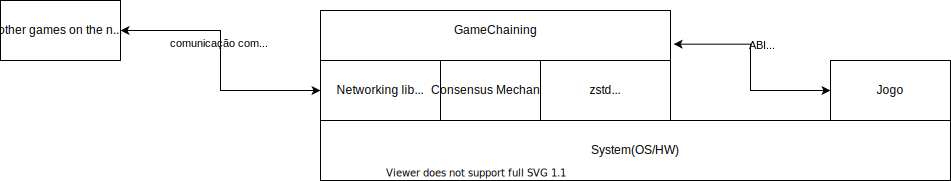
\includegraphics[width=1\textwidth]{blockchain_comunication.png}
      \caption{Comunicações do \gamechaining{}}
      \label{fig:gamechaining_coms}
\end{figure}

\newpage
\section{Conclusões}
\label{sec:blockchain_conclusao}
Após este estudo consideraram-se os seguintes conceitos, estudados em detalhe e abordados anteriormente, para possibilitar a implementação do projeto em causa:

\begin{itemize}

      \item
            \textit{Rust} - como a linguagem de programação pelas razões já referidas em \ref{subsection:rust}

      \item
            \acrshort{pos} - verificação de transações, em que se podem atribuir itens do inventario do utilizador em \textit{stake} \textsuperscript{\ref{concenso}}
      \item
            \textit{Sharding} - para poupar utilização de memória distribuindo a \textit{blockchain} entre múltiplos dispositivos
            \textsuperscript{\ref{sharding}}

      \item
            \textit{libp2p} - uma biblioteca a utilizar para a \textit{stack} de \textit{networking} ser mais facilmente desenvolvida

      \item
            \textit{zstd} - método de compressão em tempo real desenvolvido pelo \textit{Facebook} para rápidas descompressões \cite{zstd_github}, podendo ajudar a diminuir o tamanho que a \textit{blockchain} ocupa no disco caso seja necessário.
      \item
            \textit{Hole punching} - para não obrigar os utilizadores(ou pelo menos não todos) a terem portas abertas 

      \item
            \acrshort{ipc-compute} ou \acrshort{abi} - para comunicação com o jogo propriamente dito.

\end{itemize}

Com as opções apresentadas pode-se concluir que é possível construir o \gamechaining{} (nome dado ao projeto referido no \hyperref[anexo:A]{anexo A}) com tecnologias e algoritmos já existentes facilitando o seu desenvolvimento. 

Existem algumas preocupações sobre o espaço que pode ser ocupado no disco e os requerimentos de \textit{networking} mas podem-se limitar essas preocupações com \textit{sharding}\textsuperscript{\ref{sharding}} e compressão para resolver o problema de armazenamento e 

\textit{hole punching} para não obrigar todos os utilizadores a modificar as suas redes.

Estas modificações podem trazer preocupações pelo facto de obrigarem a um certo nível de centralização em que iria existir a necessidade de confiar num certo número de indivíduos para que funcionasse. Isto contradiz o requisito R3 mas é aceitável pois é um conceito parecido com jogos com \textit{hosts}, como \textit{Minecraft}, em que um utilizador iria ter a responsabilidade de ter um servidor pronto para outros jogarem, o que remove a centralização de uma empresa única. 

As propriedades do \gamechaining{} consideradas anteriormente ajudariam os jogadores menos proficientes tecnicamente a jogar enquanto que outros membros da comunidade mais capazes poderiam ter benefícios no jogo por ajudar a manter o jogo activo. Também podem ser feitos serviços em que um jogador aloca um espaço num servidor externo para ter a sua própria instância do serviço do jogo, como fazem algumas empresas como a \textit{Azure} e o \textit{Linode} com servidores de \textit{Minecraft}, por exemplo.

Blockchain pode ajudar em termos de estabilidade do mundo em que podem existir múltiplos \textit{hosts} para o mesmo mundo e existe a verificação e registo de mudança de dados o que pode servir como um \gls{anticheat}, podendo se criar mundos ativos muito maiores do que seria possível num jogo como \textit{Minecraft} ou outros que têm um único servidor.

Uma pesquisa intensa ajudou em muito a obter informação de como seria a aplicação desta tecnologia neste contexto. Porém, existem ainda várias questões práticas que se devem considerar e rever. Por exemplo,  ainda existem duvidas quanto à existência de servidores da comunidade para resolver os problemas referidos anteriormente.

Pelo facto de este ser um projeto mais extenso do que o esperado, como se pode observar comparando a proposta de estágio e os requisitos descritos neste capítulo, o projeto tornou se mais amplo do que inicialmente planeado, isso porque o interesse aumentou ao longo da pesquisa e nas sucessivas reuniões. 

Como não se podia concluir com certeza se haveria uma implementação para apresentar no final de estágio decidiu-se mover o estagiário para outros projetos com uma estrutura mais comum para implementar.




\chapterf{AC7ION}
\label{chap:ac7ion}
\section{Introdução}

Depois de estudado o conceito de blockchain investiu-se tempo a desenvolver uma ferramenta que teria uma estrutura parecida com o que se desejava que o \gamechaining{} fosse em termos de comunicação com os motores de jogos. Assim, o \textit{AC7ION}, tornou-se numa prova de conceito neste aspeto.

O \textit{AC7ION} é um recetor de \textit{tweets} com uma  \# (\textit{hashtag}) específica e enviando-os a um jogo que os requisite.

\section{Requisitos}

Neste projeto existiam requisitos semelhantes aos apresentados no projeto \gamechaining{}:

\begin{itemize}
	\item
	      \textbf{R1} - Deve ser agnóstico quanto ao motor de jogo e sistema operativo, isto é, não deve ter dependências ou requerimentos que o impeçam de ser usado noutras plataformas, exceto se as plataformas em questão forem muito restritas relativamente ao que se pode executar
	\item
	      \textbf{R2} - Deve ser rápido e responsivo, sem grandes requisitos relativamente à execução, isto é, evitar que se use muito \acrshort{cpu} ou memória, de forma que não afete muito o desempenho do jogo
	\item
	      \textbf{R3} - Não pode estar presa a licenças comerciais sendo possível ser de código aberto caso se queira publicar
    \item 
        \textbf{R4} - Receber os \textit{tweets} em tempo real no servidor quando estes são enviados 
    \item 
        \textbf{R5} - Guardar até x \textit{tweets} recebidos para serem enviados para o cliente
\end{itemize}

Com estes requisitos é possível fazer algo comparável com a planeada estrutura de comunicação entre um jogo e a biblioteca do \gamechaining{}.

\section{Tecnologias}

Neste trabalho aplicaram-se certos conhecimentos que se adquiriram ao longo do estudo sobre \textit{blockchain}, nomeadamente a linguagem \textit{Rust} e uma das suas bibliotecas para comunicação assíncrona designada \textit{Tokio}.

\subsection{\textit{Tokio}}

\textit{Tokio} é um \textit{runtime} assíncrono para a linguagem de programação \textit{Rust}.
O \textit{runtime} é composto por um \textit{condutor de entradas e saídas}, gestor de tarefas, temporizador e uma piscina de bloqueamento, em que todos estes mecanismos juntos criam uma camada para gestão e execução, de forma assíncrona, de tarefas.

Foi criada para ocupar o espaço que faltava na \acrshort{std} no espaço de funções assíncronas e o \textit{runtime} para as executar concorrentemente, chegou a uma versão estável em janeiro de 2021. Esta pode ser usada em vários sistemas incluindo sistemas embutidos ou grandes servidores com vários cores em que a biblioteca escala-se bem sem grande esforço do programador.

Facilita o desenvolvimento de programas eficientes e concorrentes de redes graças às funcionalidades do \textit{Tokio} com \textit{Rust} já descritas anteriormente. \cite{rust-fearless}

\subsection{Outras bibliotecas usadas}

Para que o servidor consiga comunicar com a \acrshort{api} do \textit{Twitter} usou se a biblioteca \textit{egg-mode} que foi desenvolvida para esse propósito. \cite{egg-mode_github}
\textit{Egg-mode} foi escolhida por ter a maior popularidade no \textit{github} e pela facilidade de utilização.

Para serialização e desserialização de \acrshort{json} usaram-se os pacotes \textit{serde} e \textit{serde\_json}. Estas bibliotecas foram usadas para converter \textit{tweets} recebidos no formato \acrshort{json} para serem enviadas aos motores de jogo.

Para aspetos de data e hora foi usada a biblioteca \textit{chrono}. Esta era usada para desenvolver operações como verificar as idades dos \textit{tweets}, tempos de envio, etc.

Para constantes e funções do padrão de \textit{C} usou-se a biblioteca \textit{libc}. Esta serviu para criar as funções que iriam ser usadas por \acrshort{abi} pelos motores de jogo.

Para uma implementação de estruturas de sincronização mais rápidas do que as existentes na \acrshort{std} usou-se a biblioteca \textit{parking\_lot}. Esta demonstrava melhores resultados na estrutura \textit{mutex}, uma estrutura que guarda um recurso para que seja usado entre linhas de execução para prevenir condições de corrida. \cite{parking_lot_benchmarks}

Para abstrações de programação assíncrona foi usada a biblioteca \textit{futures}. Esta foi utilizada para fazer operações em iteradores assíncronos, como a \textit{stream} de \textit{tweets} em que usou-se 

para processar cada \textit{tweet} individual.

\section{Ferramentas}

Para desenvolvimento usou-se \textit{Clion}. Um \acrfull{ide} criado pela \textit{JetBrains}, com o objetivo de ser um \acrshort{ide} para \textit{C/C++}. A \textit{JetBrains} publica na loja de \textit{plugins} do \textit{Intellij} e \textit{Clion} o \textit{plugin} \textit{Rust} para adicionar suporte para desenvolvimento deste nestes \acrshortpl{ide} como demonstrado na \cref{fig:devenv}. 

\begin{figure}[H]
    \centering
    \includegraphics[width=\textwidth]{images/devenv-rust.png}
    \caption{Ambiente de desenvolvimento: \textit{Clion} com o \textit{plugin} para \textit{Rust}}
    \label{fig:devenv}
\end{figure}

\section{Arquitetura}

Usa-se um modelo servidor-cliente, em que um servidor se coneta com as \acrshortpl{api} do \gls{twitter}, recebem-se os \textit{tweets} necessários e enviam-se para os clientes que seriam bibliotecas partilhadas para os jogos usarem.

Na prática os jogos fazem o pedido de x \textit{tweets} e o cliente faz o pedido ao servidor para receber as
informações num formato de \acrshort{json}, sendo que no lado do jogo não é necessário preocupações com qualquer funcionalidade de \textit{networking}.

Na \cref{fig:twitter_arq} podemos ver de uma forma mais visual como tudo está conectado.

\begin{figure}[!ht]
  \centering
  \includegraphics[width=0.9\textwidth]{twitter}
  \caption{Arquitetura do \textit{AC7ION}}
  \label{fig:twitter_arq}
\end{figure}


O server é \textit{multithreaded} e assíncrono, o que significa que ele irá usar automaticamente todos os \textit{cores} do \acrshort{cpu} do sistema em que está a ser executado. O programa também é \textit{memory safe} e não tem \glspl{data-race} já que a verificação destes problemas são verificados em tempo de compilação. \cite{rust-fearless}

\newpage
\section{Conclusão}

Com o objetivo de testar a arquitetura pretendida para o \gamechaining{}, completou-se o \textit{AC7ION} num espaço de 2 semanas. Este projeto comprovou a viabilidade desta arquitetura, proporcionando mais experiência ao estagiário em \textit{blockchain} e na criação de bibliotecas para motores de jogos de vídeo.



\chapterf{Detector de batimentos cardíacos para a \textit{Nintendo Switch}}
\label{chap:bpm}

\section{Introdução}

Como tarefa pré-final, foi realizada a missão de experimentar desenvolvimentos para consolas de jogos, tendo-se a ideia de fazer um detetor de batimentos cardíacos
para a \gls{switch} e um jogo com ele designado de \textit{DMS}. Para este projeto, o único requisito era o de detetar os batimentos cardíacos de alguém com o polegar no sensor.

\section{Nintendo Switch}

A \gls{switch} (\cref{fig:switch}) é uma consola de jogos de vídeo híbrida produzida pela empresa \textit{Nintendo} com várias funcionalidades inovadoras no mercado, aspeto que caracteriza esta bem conhecida empresa.

Existem várias funcionalidades nesta consola não muito comuns noutras, como por exemplo dois comandos removíveis nas laterais, designados \textit{Joy-Cons}, podendo ser usados como comandos individuais ou como um só em conjunto.

Em ambos existem botões que se espelham um ao outro na sua quase totalidade, exceto alguns botões com funções especiais para servirem de comandos individuais quando necessário. Ambos têm um giroscópio e um acelerómetro para rastrearem movimentos; existe um \acrfull{nfc} no \textit{Joy-Con} esquerdo e um sensor de \acrshort{ir} no lado direito, este ultimo é aquele que vai ser utilizado para o \textit{DMS}.

\begin{figure}
  \centering
  \includegraphics[width=0.9\textwidth]{switch}
  \caption{\gls{switch} \cite{switch_info}}
  \label{fig:switch}
\end{figure}



\section{DMS}

O \textit{DMS} é um jogo, desenvolvido pela \textit{Nerd Monkeys}, cujo o objetivo é o de um jogador, que esteja a segurar num \textit{Joy-Con} direito com o polegar em cima do sensor (ver \cref{fig:switch_irsensor}), tentar manter a calma enquanto outros jogadores tentam aumentar o ritmo cardíaco do outro jogador. Isto pode ser conseguido da forma que acharem mais apropriada, com historias ou mecanismos que assustem ou destabilizem o outro jogador (ex: fazer cócegas).

No contexto do jogo, o estagiário ficou responsável por fazer o detetor de batimentos cardíacos de forma a tornar esta ideia possível.

\newpage
\section{Sensor de IR}

\begin{wrapfigure}{R}{5cm}
  \centering
  \includegraphics[width=5cm]{switch_irsensor.png}
  \caption{\acrshort{ir} \textit{Sensor} da \gls{switch} \cite{switch_irsensor_source}}
  \label{fig:switch_irsensor}

\end{wrapfigure}


O \textit{input} do sensor de \acrshort{ir} pode ser facilmente acedido por uma aplicação ou biblioteca na consola, de varias formas possíveis.

Existem várias formas de usar o sensor mas a forma mais conveniente é detetar a intensidade da luz recebida, o que pode ser usado para detetar a quantidade de oxigénio no sangue que passa no polegar. O tempo que demora entre a intensidade de subir e descer pode ser vista como o tempo de um batimento, com este tempo pode-se calcular os batimentos por minuto.

\section{Arquitetura}

Pode-se observar na \cref{fig:bpm_arch} a arquitetura do projeto, que este é desenvolvido de forma independente do jogo. O jogo só necessita de incluir a biblioteca e chamar a função para atualizar os dados, recomenda-se que esta seja chamada 60 vezes por segundo ou numa frequência superior para uma melhor deteção do valor.

\begin{figure}[H]
  \includegraphics{batimentos}
  \caption{Arquitetura do sensor de batimentos cardíacos}
  \label{fig:bpm_arch}

\end{figure}

\newpage
\section{Tecnologias e ferramentas usadas}

Para o desenvolvimento desta biblioteca utilizou-se as ferramentas referidas na \cref{tab:bpm_software}.

\begin{table}[H]
  \centering
  \begin{tabularx}{\linewidth}{lCC}
    \multicolumn{1}{c}{\textbf{Nome}}                                       &
    \multicolumn{1}{c}{\textbf{Descrição}}                                  &
    \multicolumn{1}{c}{\textbf{Utilização no projeto}}
    \tabularnewline \tabularnewline
    C++                                                                     &
    Uma linguagem de programação compilada multi-paradigma e de uso geral.  &
    Linguagem usada para programar a biblioteca.
    \tabularnewline \midrule
    \textit{Nintendo SDK}                                                   &
    Ferramentas usadas para desenvolver para sistemas da \textit{Nintendo}. &
    Usadas para acessar as \acrshortpl{api} da \gls{switch} e compilar a biblioteca.
    \tabularnewline \midrule
    \textit{Visual Studio}                                                  &
    Um \acrshort{ide} criado pela \textit{Microsoft}.                       &
    Usado para executar e testar código.
    \tabularnewline \midrule
    \textit{Clion}                                                          &
    Um \acrshort{ide} criado pela \textit{JetBrains}.                       &
    Usado como principal ambiente de desenvolvimento para escrever o algoritmo.
    \tabularnewline \midrule
  \end{tabularx}
  \caption{Tecnologias e ferramentas usadas no detector de batimentos cardíacos}
  \label{tab:bpm_software}
\end{table}

\section{Implementação}

Para a implementação houve 3 etapas principais para o sucesso deste projeto sendo estas a  \nameref{sec:recpdados}, a \nameref{sec:normalizacao} e por último \nameref{sec:ciclos}.

\subsection{Receção de dados}
\label{sec:recpdados}

O processo começou por conseguir detetar batimentos com o sensor que não pode ser descrito.

Depois de se conseguir quando obtêm-se os valores corretos para detetar batimentos, usou-se a média total da intensidade de luz refletida como um valor único de input da câmara e o tempo passado desde que o programa começou.

Como tal, fez-se um gráfico na consola para verificar os valores, obtendo-se o que se pode ver na \cref{fig:rawdata}.

\begin{figure}[H]
  \centering
  \includegraphics[width=\textwidth]{rawdata}
  \caption{Gráfico com as intensidades ao longo do tempo.}
  \label{fig:rawdata}
\end{figure}

\subsection{Normalização do gráfico}
\label{sec:normalizacao}
Como se pode observar, o gráfico obtido era difícil de analisar. Então, decidiu-se fazer um simples algoritmo de normalização, em que cada ponto seria a média dos últimos 10 pontos. Desta forma conseguiu-se um gráfico melhorado, apresentado na \cref{fig:normalized}.


\begin{figure}[H]
  \centering
  \includegraphics[width=\textwidth]{normalized}
  \caption{Gráfico com as intensidades normalizadas.}
  \label{fig:normalized}
\end{figure}

Com este simples método de normalização conseguem-se gráficos mais fáceis de analisar, cada vez maior for o número de pontos na media menos pontos existem que saltam tanto mas mais tempo demora a ter se valores usáveis e cada vez mais o gráfico fica com picos mais suaves, o que torna mais difícil descobrir as zonas de picos.


\subsection{Deteção de ciclos}
\label{sec:ciclos}
Um ciclo neste contexto consiste na passagem por um mínimo no gráfico, passando por um máximo e finalizando com um mínimo novamente,isto é considerado em termos práticos um batimento.

Concluindo, para calcular os batimentos por minuto faz-se a média das durações dos últimos ciclos.

\section{Testes}

\begin{wrapfigure}{r}[1cm]{2cm}
  \centering
  \includegraphics[height=2cm]{smartwatch.png}
  \caption{\textit{Smartwatch} com \acrshort{ir} \cite{smartwatch}}
  \label{fig:smartwatch}
\end{wrapfigure}

A biblioteca foi testada com uma pequena amostra de pessoas.
A amostra era de 5 pessoas, 2 crianças e 3 adultos. O sensor conseguia detetar o batimento, pelo polegar da amostra completa.

Comparou se os valores obtidos com o que o sensor de batimentos de um \textit{smartwatch} (\cref{fig:smartwatch}) em que se concluiu que o algoritmo desenvolvido obtinha valores inferiores ao do relógio ao redor de 10 a 20 batimentos por segundo.

A vantagem do algoritmo desenvolvido é ter um tempo de resposta a mudanças de batimento muito mais rápida o que é favorável para o jogo a ser desenvolvido.

\section{Conclusão}

A biblioteca não reporta números fiáveis para uma
deteção precisa dos batimentos por minuto de uma pessoa que a usa. Porém, serve perfeitamente para saber quando o batimento sobe ou desce, o que pode ser muito bem utilizado num jogo, principalmente para o \textit{DMS}.

Concluído este projeto, o estagiário ganhou experiência com a \gls{switch} e ganhou conhecimentos sobre o seu funcionamento e regras de utilização.



\chapter{Conclusão}
\label{chap:conclusao}
Dando o estágio por terminado, é necessário fazer um balanço do que foi conseguido, tanto na perspetiva
do estagiário como da empresa, e do que será necessário e prioritário desenvolver no futuro para que o projeto desenvolvido evolua. É este o objetivo do presente capítulo.

\section{Objetivos Atingidos}
 
Com a chegada das criptomoedas e a sua exploração e popularidade houve um crescente interesse por \textit{blockchain} e suas áreas de aplicação. 

A \textit{Nerd Monkeys} é uma das várias empresas que tiveram interesse no assunto e fizeram a proposta de estágio para que o estagiário, João Gonçalves, estudasse a matéria em causa e chegasse as suas conclusões sobre ela.

O processo estava a correr bem mas estava a ser mais longo do que o esperado, impossibilitando o cumprimento do plano dentro de previsto. Assim, seria previsível que o estagiário acabasse o estágio sem qualquer implementação feita pelo que se decidiu mudar os planos e propor ao estagiário a realização de outras tarefas que mostrassem a sua capacidade de implementação e que  aplicassem alguns conhecimentos que podiam interessar ao presente estudo.

O primeiro foi o \textit{AC7ION}, este ajudou o estagiário a ganhar experiência com Rust e como fazer bibliotecas para motores de jogo. Houve um período em que se testava qual a forma correta de fazer \acrshort{abi} com \textit{C++} e \textit{Rust} para testar como alguns motores de jogos reagiam e desenvolvendo-se o \textit{AC7ION}.

De seguida desenvolveu se a biblioteca para o \textit{DMS} com bons resultados.

Concluindo, as investigações e desenvolvimentos feitos nesta área durante o estágio, do ponto de vista dos interesses da empresa nesta temática, obteve resultados positivos o que fez com que o estágio fosse um sucesso.

\section{Desenvolvimentos Futuros}

O \gamechaining{} é um projeto que tanto a \textit{Nerd Monkeys} como o estagiário querem continuar por isso será algo que vai se retomar quando considerado oportuno. Enquanto isso o estagiário vai continuar a trabalhar com a \textit{Nerd Monkeys} em outros projetos.

\printbibliography[heading=bibintoc]
\label{bibliografia}
% ===== ANEXOS =====

\chapterf{Anexos}
\label{chap:anexos}
 % anexo A
\newcommand{\anexoA}{Anexo A - Proposta de Estágio}
\part*{\anexoA}
\label{anexo:A}
\addcontentsline{toc}{section}{\anexoA}
\includepdf[pages=-]{proposta.pdf}

\end{document}
